\documentclass{article}
\usepackage{graphicx}
\usepackage[margin=1.5cm]{geometry}
\usepackage{amsmath}

\begin{document}

\title{Monday Reading Assessment: Unit 8, Momentum}
\author{Prof. Jordan C. Hanson}

\maketitle

\section{Memory Bank}

\begin{itemize}
\item $\vec{p} = m\vec{v}$ ... Definition of momentum.
\item $\vec{p}_{\rm total} = \vec{p}_1 + \vec{p}_2$ ... Total momentum is the sum of two momenta.
\item $\vec{p}_{\rm total,i} = \vec{p}_{\rm total,f}$ ... Momentum is conserved, like energy.
\item $KE_{\rm Ti} = KE_{\rm Tf}$ ... Kinetic energy conservation (elastic collisions).
\item $m_p = 1.67 \times 10^{-27}$ kg ... Mass of protons.
\end{itemize}

\section{Momentum}

\begin{enumerate}
\item
\begin{figure}[ht]
\centering
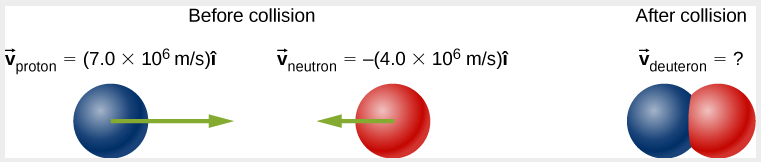
\includegraphics[width=0.75\textwidth]{deuteron.png}
\caption{\label{fig:deu} One car bumps another.}
\end{figure}
A proton collides with a neutron (with essentially the same mass as the proton) to form a particle called a deuteron. What is the velocity of the deuteron if it is formed from a proton moving with velocity $7.0 \times 10^{6}$ m/s to the right and a neutron moving with velocity $-4.0 \times 10^{6}$ m/s to the left? \\ \vspace{2cm}
\item Check whether or not kinetic energy is conserved.  (a) What is the initial total kinetic energy? (b) What is the final total kinetic energy?
\end{enumerate}
\end{document}
